%! TeX program = pdflatex
%! TeX TS-program = pdflatex

\documentclass[10pt]{IEEEtran}
\usepackage{amsmath}
\usepackage[utf8]{inputenc}
\usepackage{fontenc}
\usepackage{dirtytalk}
\usepackage[dvipsnames]{xcolor}
\usepackage{tikz}
\usepackage{varwidth}
\usepackage{listings}
\usepackage{graphicx}
\usetikzlibrary{positioning}
\tikzset{
  x=1em,
  y=1em,
}
\lstset{
  basicstyle=\ttfamily\footnotesize,
  showstringspaces=false,
  commentstyle=\itshape,
  keywordstyle=\bfseries\color{cyan},
  stringstyle=\ttfamily,
  language=C,
  tabsize=2,
  breaklines=true,
  breakatwhitespace=true,
  escapeinside={\%*}{*)},
  morekeywords={
    cv,
    filter2D,
    abs,
    NORM_MINMAX,
    CV_8UC1,
    THRESH_BINARY,
    threshold,
    Point,
    BORDER_DEFAULT,
    normalize,
    equalizeHist
  },
}

\graphicspath{{code/res/}}

\title{Encontrando el \say{esqueleto} de un dibujo}

\author{ Brandon Marquez Salazar }

\begin{document}
  \maketitle
  \section{Introducción}
  En este documento se muestra el procedimiento en el que se pueden encontrar los trazos básicos de un dibujo o su "esqueleto". Este es un problema típico que se puede encontrar en el área de artes digitales
  el momento de querer digitalizar, esbozar o mejorar una imagen.

  \section{Materiales y métodos}
  El programa se realizará utilizando el lenguaje C++ y la biblioteca OpenCV para la manipulación de gráficos.

  Para este trabajo, se probarán dos métodos. El primero consta de mejorar la imagen antes de su procesamiento, resaltando ciertos relieves,
  mientras que el segundo consiste en el mejoramiento de la imagen póstumo a la detección de los bordes.

  Para realizar este proceso se propuso el uso de un kernel de $3\times3$ de la forma

  \begin{center}
    \begin{tabular}{ c c c }
      -2 & -2 &  0\\
      -2 &  0 & -2\\
      0 & -2 & -2
    \end{tabular}
  \end{center}

  El cual se puede aplicar mediante OpenCV a una imagen de 1 canal. Y dado que las imágenes proporcionadas son de más de un canal,
  estas deberán ser convertidas a escala de grises para su correcto procesamiento.

  ¿Por qué no se utilizó Canny?, esto es debido a que el Kernel seleccionado confiere una respuesta menos sensible al ruido; a comparación de
  Canny que suele ser más sensible.

  \section{Objetivos}
  El objetivo principal es la extracción de los trazos básicos de un dibujo o su "esqueleto" a través de la detección de bordes.
  El objetivo secundario de este trabajo es la comparación de resultados obtenidos al aplicar el filtro de detección sin un mejoramiento
  previo a la detección de bordes respecto a los obtenidos al aplicar un mejoramiento previo a la detección de bordes.


  \section{Procedimiento}
  Inicialmente, las imágenes son cargadas al programa mediante el método \texttt{imread(std::string path, int flag)}. Proporcionando desde
  este momento que se utilizará el espacio en escala de grises.

  Una vez cargada la imagen, se procede al realizar ambos procesamientos y a la obtención de resultados.
  Para ello, los métodos seleccionados fueron:
  \lstinputlisting[linerange={35-37,39}]{code/src/dibujo.cxx}

  El mejoramiento es la normalización y la umbralización. Sin embargo, este último es omitido en caso de que la imagen de entrada cuyo histograma 
  haya sido previamente igualado.
  \lstinputlisting[linerange={12}]{code/src/dibujo.cxx}

  \section{Resultados}
  Para las diferentes imágenes, se logró observar que el resultado era más limpio (aunque perdía bastante información) si se realizaba una igualación
  de histograma previo a la detección de bordes. Esto es un resultado que deja únicamente lo más resaltante de una imagen, a cambio de la perdida de
  cualquier detalle con poca variación respecto a su vecindario. Por otro lado, si la igualación de histograma no se realizaba, era necesario umbralizar,
  lo que permite tener mayor control sobre los bordes resultantes en la imagen final.

  \begin{figure}[!ht]
    \includegraphics[width=0.6\linewidth]{imagen}
    \caption{Imagen de prueba}

    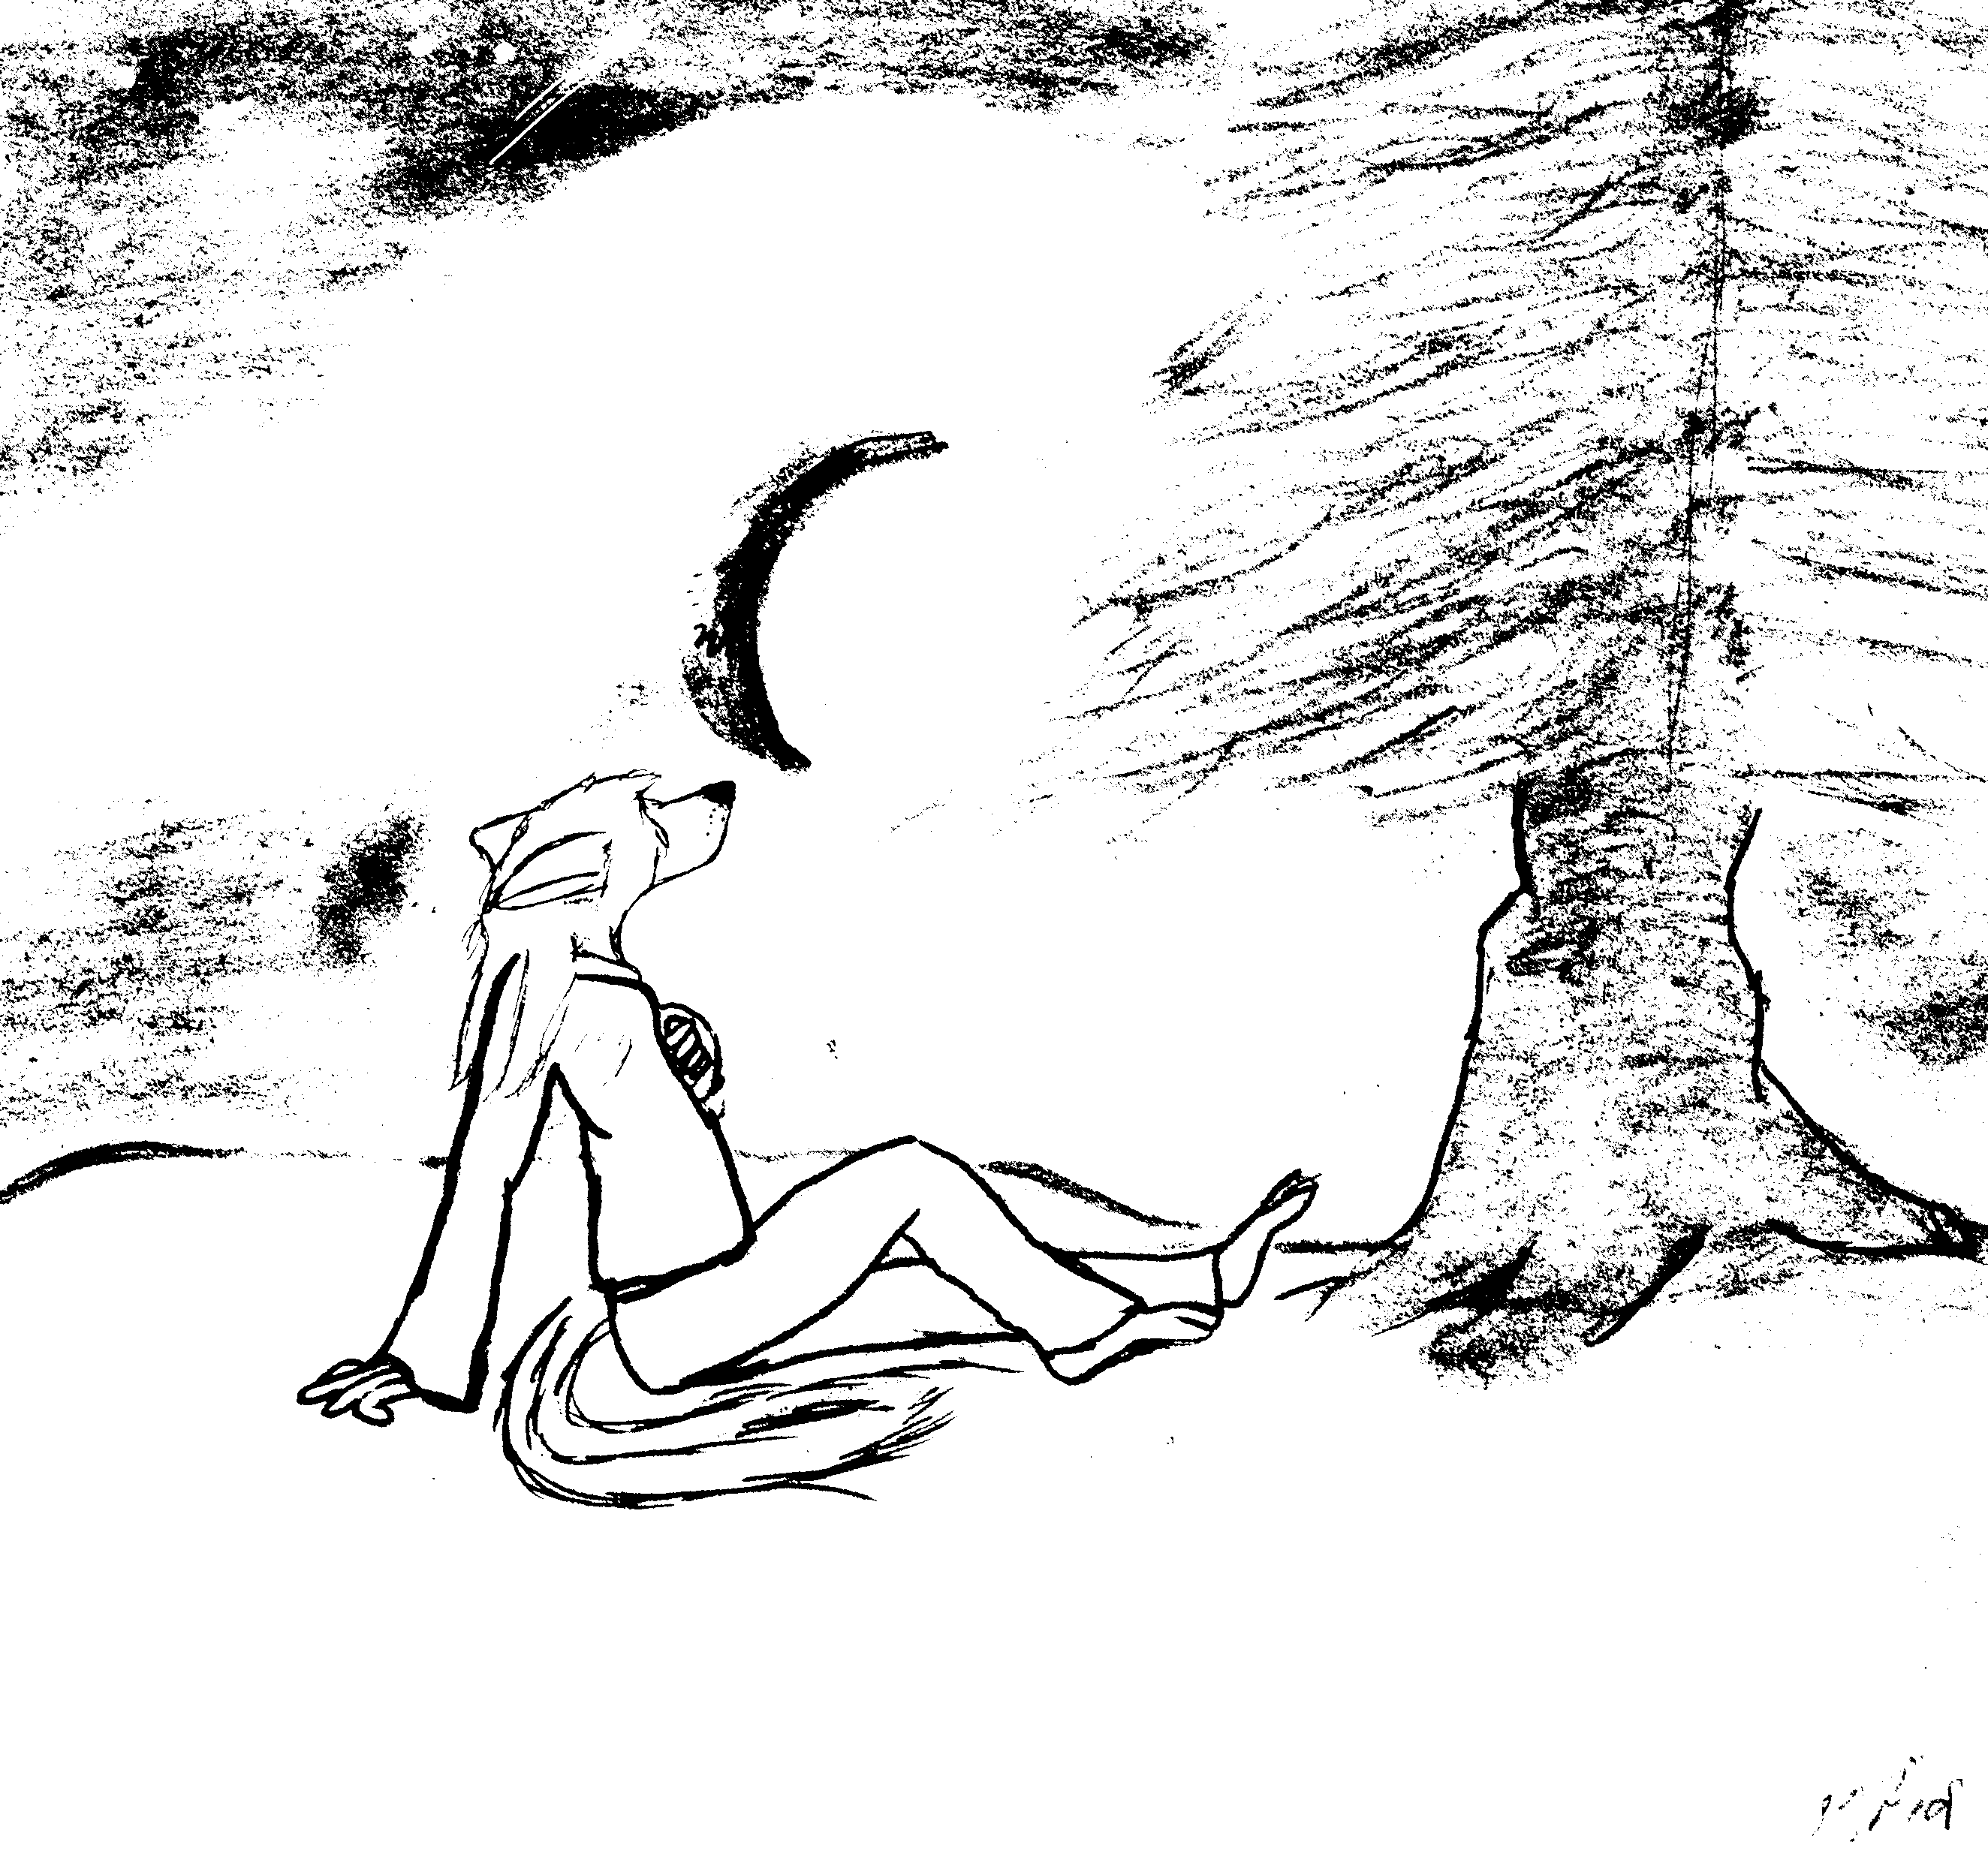
\includegraphics[width=0.6\linewidth]{salida/imagen.png_Edge.png}
    \caption{Sin igualación de histograma}

    \includegraphics[width=0.6\linewidth]{salida/imagen.png_Equalized - Edge.png}
    \caption{Con igualación de histograma}
  \end{figure}

\end{document}
